
\documentclass[conference]{IEEEtran}

\usepackage[T1]{fontenc}
\usepackage{cite}
\usepackage{graphicx}
\usepackage{booktabs}
\usepackage{multirow}
\usepackage{amsmath}
\usepackage{url}
\usepackage{hyperref}
\usepackage{algorithm}
\usepackage{algpseudocode}
\usepackage{xcolor}

\hypersetup{
  colorlinks=true,
  linkcolor=black,
  urlcolor=black,
  citecolor=black
}
\newcommand{\todo}[1]{\textcolor{red}{\textbf{[TODO: #1]}}}

\algrenewcommand\algorithmicrequire{\textbf{Input:}}
\algrenewcommand\algorithmicensure{\textbf{Output:}}

\title{Branch Prediction Simplification for AI Workloads}

\author{
\IEEEauthorblockN{Simon Darota, Winner Abula}
\IEEEauthorblockA{
Department of Computer Science\\
Khalifa University\\
Abu Dhabi, UAE\\
\{100067950, 100066896\}@ku.ac.ae
}
}


\begin{document}
\maketitle

\begin{abstract}

State-of-the-art branch predictors usually achieve high accuracy by combining multiple history lengths, tags, specialized update logic, and auxiliary correction techniques. This kind of design mechanism can be justified for general purpose complex workloads, however, it may not be necessary for AI workloads whose control flow is usually filled with regular iterative spaces.
In this project, we study whether a simpler loop-aware branch predictor is able to support competitive performance on AI based workloads simultaneously reducing predictor complexity and storage. To prove this point, we created a gem5-based evaluation pipeline for RISC-V O3CPU and compared low-complexity baseline predictors (BiModeBP and GshareBP) with advanced high-complexity predictor (TAGE). We also built a new Loop-Aware Branch Predictor (LABP) specifically tailored to AI workloads and compared its performance with the three baseline branch predictors on two representative AI microbenchmarks: a sparse-inference MLP (\texttt{tinymlp}) and a dense matrix multiplication kernel (\texttt{matmul}). Results show that TAGE remains far superior in terms of both Instructions Per Cycle (IPC) and misprediction rate across both workloads (IPC of 2.66 and 1.74 respectively, with misprediction rates below 0.25\%). LABP matches GshareBP on \texttt{tinymlp} but shows measurable gains on the loop-dominated \texttt{matmul} kernel, where its loop component achieves 98.5\% accuracy when active. These results demonstrate that loop-awareness alone is insufficient for workloads with significant data-dependent branching, but can be effective on purely loop-dominated kernels when confidence gating is conservative. This report defines the problem, explains and critiques existing approaches, presents the evaluation pipeline, and provides quantitative findings with analysis of the trade-offs involved.
\end{abstract}

\section{Problem Description}
In computer architecture, branch predictor is a digital circuit that attempts to guess which way a branch (for example, if-then-else statement) will go prior to this is known for sure. A wrong-path fetch decision wastes front-end bandwidth, pollutes speculation and reduces effective instruction throughput, hence, conditional branch prediction remains critical to high-performance processors. In deep and wide out-of-order pipelines in which a single misprediction can make substantial speculative work obsolete, the penalty is especially severe. For this reason, modern branch predictors are no longer just small counter tables, they are sophisticated multi-component designs with long histories and explicit-anti-aliasing techniques~\cite{smith_1981,yeh_patt_1992,mcfarling_1993,seznec_michaud_2006}.

This evolution creates a lot of tension. High-complexity predictors like TAGE and its derivatives achieve very high accuracy across variety of workloads, however, they also require multiple tagged tables, allocation policies that are nontrivial, heuristics that are update and extra storage ~\cite{seznec_michaud_2006,seznec_2016}. That complexity is usually justified for a general-purpose complex core. The answer is less obvious for AI based workloads. The kernels in dense linear regression models or deep neural-network inference are put together as regular loop nests. A simpler predictor may recover most of the achievable prediction performance at lower implementation cost if their dynamic branch stream is dominated by highly biased loop branches. 

The central question of this project is therefore:
\begin{quote}
\emph{Can a lightweight, loop-aware branch predictor achieve competitive accuracy and performance on AI workloads relative to conventional predictors such as bimodal, gshare, and TAGE, while reducing predictor complexity and conditional predictor storage?}
\end{quote}

This question matters for two main reasons. First, branch prediction is an energy-sensitive structure because it is consulted every cycle on the fetch path. Second, AI-oriented processors and energy-constrained systems benefit disproportionately from simpler structures when performance loss is small. Our hypothesis does not invalidate the necessity of complex predictors totally; it rather emphasizes the fact that the control-flow structure of some AI workloads may justify the need for a more specialized design.

This project contract motivated a loop-aware predictor for exactly this scheme. The intended target is a workload in which loop-exit branches are common, strongly patterned, and potentially predictable with much less machinery than a general-purpose tagged predictor. This report evaluates that hypothesis through a gem5 implementation and a two-workload benchmark study.

\section{Related Works}
Branch prediction research offers a spectrum of design points, from very small tables to highly specialized hybrid mechanisms. This section reviews the most relevant approaches and identifies what each does well, where it breaks down, and why it matters for AI-oriented control flow.

\subsection{Bimodal Predictors}
The bimodal predictor is the canonical low-complexity baseline: a table of saturating counters indexed by branch PC bits~\cite{smith_1981}. Its strengths include being compact, fast, straightforward to verify, and effective on strongly biased branches. When simplicity is our design goal, these properties make it attractive.

It is also not without a weakness. Bimodal prediction cannot exploit inter-branch correlation and is highly vulnerable to aliasing. Once multiple branches map to the same entry, unrelated behavior interferes destructively. As a result, bimodal designs generally perform poorly on branches whose outcomes depend on recent path history rather than fixed bias. 

For this project, bimodality is valuable as a floor: if a proposed simplified design cannot consistently outperform a small bimodal table on the target workload class, the simplification argument is weak.

\subsection{Two-Level Adaptive Predictors and Gshare}
Two-level adaptive predictors extended the field by introducing explicit branch history into the indexing function~\cite{yeh_patt_1992}. Gshare is the classic practical instance: it XORs global history with PC bits to reduce destructive interference while preserving low implementation overhead~\cite{mcfarling_1993}. Compared to bimodal, gshare captures correlation among branches, and it usually provides better accuracy with trade off on mixed workloads.

The limitation is that its effectiveness depends on whether useful correlations fit within the available history and table budget. When history is too short, difficult branches remain unresolved. In addition to that, when the budget is small, aliasing remains substantial. More importantly for AI workloads, gshare is agnostic to loop semantics. It benefits from repeated patterns, but it does not explicitly represent iteration count or loop confidence. Thus, it can still mispredict loop exits that are regular in a semantic sense but difficult to encode in a short global-history pattern.

\subsection{Hybrid and Interference-Reducing Predictors}
Hybrid prediction emerged to address the fact that no single mechanism works best for all branches. Tournament-style combinations and related designs select among multiple predictors so that different components specialize on different branch classes~\cite{mcfarling_1993}. Work on correlated branch prediction also highlighted how interference, rather than pure table size, often limits accuracy~\cite{young_1995}. These designs are critical as they show that moderate increment in complexity can bring substantial gains over a single predictor table.

Their drawback, from the perspective of this project, is that they move the design away from the simplicity notion. Hybrid predictors require extra tables, a selector, and more involved update logic. They often represent an effective engineering compromise, but they do not answer the narrower question posed here: whether a predictor can be simplified specifically for loop-heavy AI kernels rather than made more general.

\subsection{Tagged Predictors}
Tagged predictors deal with aliasing more directly. Michaud's tag-based work and the later TAGE design established a highly influential design principle: maintain predictor components indexed with different history lengths and use partial tags so the predictor can match the right context while limiting destructive interference~\cite{michaud_2005,seznec_michaud_2006}. TAGE is especially effective because it can use short history for easy branches and long history for difficult ones, with tagging providing robustness that simple two-level predictors lack.

For our purposes, TAGE is the strongest reference design. Its primary advantage is breadth: it delivers high accuracy across diverse branch behaviors, including branches that require distinct correlation depths. The limitation is complexity. TAGE requires multiple tagged tables, usefulness tracking, allocation and replacement logic, and a careful update policy. Since our study is centered on simplicity, TAGE will be our performance scale instead of implementation point.

\subsection{Loop Predictors}
Loop predictors exploit a specific regularity that other predictors only learn indirectly: the repeated not-taken/taken structure of counted loops. By tracking loop trip count, confidence, and iteration progress, a loop predictor can remove the persistent loop-exit mispredictions that remain even under strong global-history schemes~\cite{seznec_2016}. This is the mechanism that motivates this project.

What is good about loop prediction is also its main limitation. It is excellent when the branch stream actually contains stable counted loops, but is narrow in scope. A loop predictor can only help when it detects the right structure, maintains confidence correctly, and overrides the base predictor conservatively. On branches driven by input sparsity, activation patterns, or other data-dependent conditions, loop-awareness provides little value and can become harmful if override logic is too aggressive. Thus, loop prediction is promising for AI workloads only if those workloads are truly dominated by regular loop control rather than merely containing loops.

\subsection{Perceptron and Neural Predictors}
Perceptron-based branch prediction extended the field in a different direction by learning long-range correlations using weight vectors and dot products~\cite{jimenez_lin_2001,jimenez_lin_2002}. These methods can outperform table-based predictors based on shorter histories in branches with complex dependence on distant history.

For this project, neural predictors serve mainly as a contrast case. They reinforce a broader lesson from the literature: strong accuracy on arbitrary workloads usually requires more machinery, not less. Although perceptron predictors are conceptually elegant, they increase hardware complexity and are not aligned with the project's simplification objective. Their existence strengthens the relevance of our question by showing how far the field has moved toward complexity in pursuit of generality.

\subsection{Recent Perspective and Relevance to AI Workloads}
Recent work continues to emphasize the trade-off between predictor accuracy, storage efficiency, and implementation cost in contemporary RISC-V settings~\cite{sutar_guinde_2025}. At the same time, workload characterization studies show that branch predictability varies significantly across programs and inputs; the branch stream cannot be inferred from application labels alone~\cite{vikas_gratz_jimenez_2025}. This is the key caution for AI-oriented prediction. Dense kernels may be dominated by regular loops, but sparsity, conditional execution, and data-dependent pruning can introduce branches that are neither highly biased nor easily modeled by loop trip counting. A simplified predictor is therefore plausible only for a subset of AI workloads, not by default for all of them.

\section{Proposed Solution}
The proposed design is a \textbf{Loop-Aware Branch Predictor (LABP)} intended to occupy a narrower but simpler design point than TAGE. The architecture has three components:

\begin{enumerate}
    \item \textbf{Base predictor:} a small PC-indexed bimodal table of 2-bit saturating counters.
    \item \textbf{Loop predictor:} a compact loop structure that tracks candidate loop branches, iteration count, and confidence.
    \item \textbf{Override policy:} the loop predictor may override the base prediction only when it has a valid and sufficiently confident loop prediction.
\end{enumerate}

The underlying hypothesis is targeted and specific rather than universal. If the dominant hard branches in an AI kernel are loop exits, then explicit loop tracking should remove many mispredictions. This would otherwise require a larger general-purpose predictor. A bimodal base is retained because it is simple, fast, and adequate for strongly biased non-loop branches. The loop component is meant to add specialization without expanding into a full hybrid tagged design.

\subsection{Implementation Strategy in gem5}
LABP was implemented directly in gem5 as a new \texttt{ConditionalPredictor}. The predictor logic is defined in new source files under the branch-prediction subsystem, compiled through gem5's build system, and exposed through the Python configuration layer so that runs can be selected with \texttt{--bp-type=LAP}. The evaluation flow uses the same gem5 O3CPU configuration for all predictors in order to isolate branch-prediction effects. Metrics are extracted from \texttt{stats.txt}, while conditional predictor storage is estimated from generated \texttt{config.ini} parameters.

In our design we reuse gem5's loop-predictor support rather than re-implementing loop tracking from scratch. This keeps the proposed predictor modular and allows the study to focus on the composition of a simple base predictor with a loop-aware override. The main research question is therefore not whether loop prediction can be implemented, but whether this particular combination is sufficient to recover a useful fraction of TAGE's performance on the target workload class.

\subsection{Predictor Pseudocode}
Algorithm~\ref{alg:lapbp} summarizes the predictor behavior at a higher level. The essential point is that LABP computes a low-cost base prediction first, then admits a loop-based override only when the loop component is confident.

\begin{algorithm}[t]
\caption{LABP lookup and update flow}
\label{alg:lapbp}
\footnotesize
\begin{algorithmic}[1]
\Require PC, thread id $tid$, actual outcome on update
\State \textbf{State:} bimodal counter table $B[0 \ldots N-1]$, loop table $L$
\Function{Lookup}{$tid, pc$}
    \State $idx \gets (pc \gg shift) \;\&\; (N-1)$
    \State $basePred \gets (B[idx] > \theta)$
    \State $(loopValid, loopPred, meta) \gets L.\textsc{Predict}(tid, pc)$
    \If{$loopValid$}
        \State $finalPred \gets loopPred$
    \Else
        \State $finalPred \gets basePred$
    \EndIf
    \State \Return $(finalPred,\{idx, basePred, meta\})$
\EndFunction
\Function{Update}{$tid, pc, actual, h, squashed$}
    \If{$h = \varnothing$}
        \State \Return
    \EndIf
    \If{$squashed$}
        \State $L.\textsc{Squash}(h.meta)$
        \State \Return
    \EndIf
    \State $L.\textsc{Update}(tid, pc, actual, h.meta, h.basePred)$
    \If{$actual = taken$}
        \State Increment $B[h.idx]$
    \Else
        \State Decrement $B[h.idx]$
    \EndIf
\EndFunction
\end{algorithmic}
\end{algorithm}

\subsection{Benchmark Workloads}
The evaluation uses two microbenchmarks selected to represent distinct points on the AI control-flow spectrum.

\textbf{tinymlp} (Algorithm~\ref{alg:tinymlp}) is a compact inference-style benchmark modelling quantised INT8 forward propagation through a two-layer MLP with magnitude-based sparsity pruning. It contains the loop nests one would expect in an MLP forward pass, but also introduces data-dependent conditions that skip work when values are zero or below a sparsity threshold. The resulting control flow is therefore mixed: regular loop branches coexist with input-dependent inner branches. This makes \texttt{tinymlp} a useful test because it probes exactly the boundary case that matters for our project: a workload that appears loop-heavy at a structural level but is not purely regular at the branch level.

\textbf{matmul} (Algorithm~\ref{alg:matmul}) performs dense $64\times64$ integer matrix multiplication repeated 20 times. Its branch stream consists almost entirely of counted-loop exits with no data-dependent conditionals inside the inner loop, making it the canonical best case for a loop-aware predictor. Comparing both workloads reveals whether simplification gains depend on loop purity.

\begin{algorithm}[t]
\caption{\texttt{tinymlp} control-flow skeleton}
\label{alg:tinymlp}
\footnotesize
\begin{algorithmic}[1]
\For{$iter = 1$ to $T$}
    \For{$i = 1$ to $H$}
        \State $acc \gets b_1[i]$
        \For{$j = 1$ to $D$}
            \If{$|x[j]| > \tau$}
                \State $acc \gets acc + W_1[i,j] \cdot x[j]$
            \Else
                \State $skipped \gets skipped + 1$
            \EndIf
        \EndFor
        \State $h[i] \gets \mathrm{ReLU}(acc)$
    \EndFor
    \For{$k = 1$ to $O$}
        \State $acc \gets b_2[k]$
        \For{$i = 1$ to $H$}
            \If{$h[i] \neq 0$}
                \State $acc \gets acc + W_2[k,i] \cdot h[i]$
            \Else
                \State $skipped \gets skipped + 1$
            \EndIf
        \EndFor
        \State $y[k] \gets acc$
    \EndFor
\EndFor
\end{algorithmic}
\end{algorithm}

\begin{algorithm}[t]
\caption{\texttt{matmul} control-flow skeleton}
\label{alg:matmul}
\footnotesize
\begin{algorithmic}[1]
\Require $N \times N$ matrices $A$, $B$; repetition count $R$
\Ensure $N \times N$ product matrix $C$; accumulated checksum
\State Initialise $A[i][j] \gets i+j$, $B[i][j] \gets 2i+j$
\For{$rep = 1$ to $R$}
    \For{$i = 1$ to $N$}
        \For{$j = 1$ to $N$}
            \State $acc \gets 0$
            \For{$k = 1$ to $N$}
                \State $acc \gets acc + A[i][k] \cdot B[k][j]$
            \EndFor
            \State $C[i][j] \gets acc$
        \EndFor
    \EndFor
    \State $checksum \gets checksum + \sum_{i,j} C[i][j]$
\EndFor
\end{algorithmic}
\end{algorithm}

\section{Results}

All experiments use gem5 in RISC-V SE mode with an O3CPU, L1/L2 caches enabled, and 10 million committed instructions per run. The analysis pipeline extracts IPC, CPI, branch predictor lookups, branch mispredictions, and an estimate of conditional predictor storage from gem5's \texttt{stats.txt} and \texttt{config.ini} files. Each predictor was evaluated on both \texttt{tinymlp} and \texttt{matmul}.

\subsection{Overall Performance}

Table~\ref{tab:results} reports per-workload metrics for all four predictors.

\begin{table}[t]
\centering
\caption{Branch predictor comparison across both workloads (RISC-V O3CPU, 10M instructions).}
\label{tab:results}
\footnotesize
\begin{tabular}{llrrrr}
\toprule
Workload & Predictor & IPC & CPI & Mispred.\ Rate & KB \\
\midrule
\multirow{4}{*}{tinymlp}
 & BiModeBP & 1.638 & 0.610 & 0.0521 & 6.00 \\
 & GshareBP & 0.974 & 1.027 & 0.0758 & 0.50 \\
 & LAP      & 0.974 & 1.027 & 0.0758 & 2.13 \\
 & TAGE     & 2.664 & 0.375 & 0.0023 & 7.94 \\
\midrule
\multirow{4}{*}{matmul}
 & BiModeBP & 1.680 & 0.595 & 0.0155 & 6.00 \\
 & GshareBP & 1.679 & 0.595 & 0.0159 & 0.50 \\
 & LAP      & 1.680 & 0.595 & 0.0157 & 2.13 \\
 & TAGE     & 1.744 & 0.573 & 0.0005 & 7.94 \\
\bottomrule
\end{tabular}
\end{table}

Figure~\ref{fig:ipc} compares IPC across predictors and workloads. On \texttt{tinymlp}, TAGE achieves an IPC of 2.66, more than $1.6\times$ the next-best predictor (BiModeBP at 1.64), while GshareBP and LAP are tied at 0.97. On \texttt{matmul}, all four predictors cluster between 1.68 and 1.74 IPC, with TAGE holding a modest lead.

\begin{figure}[t]
\centering
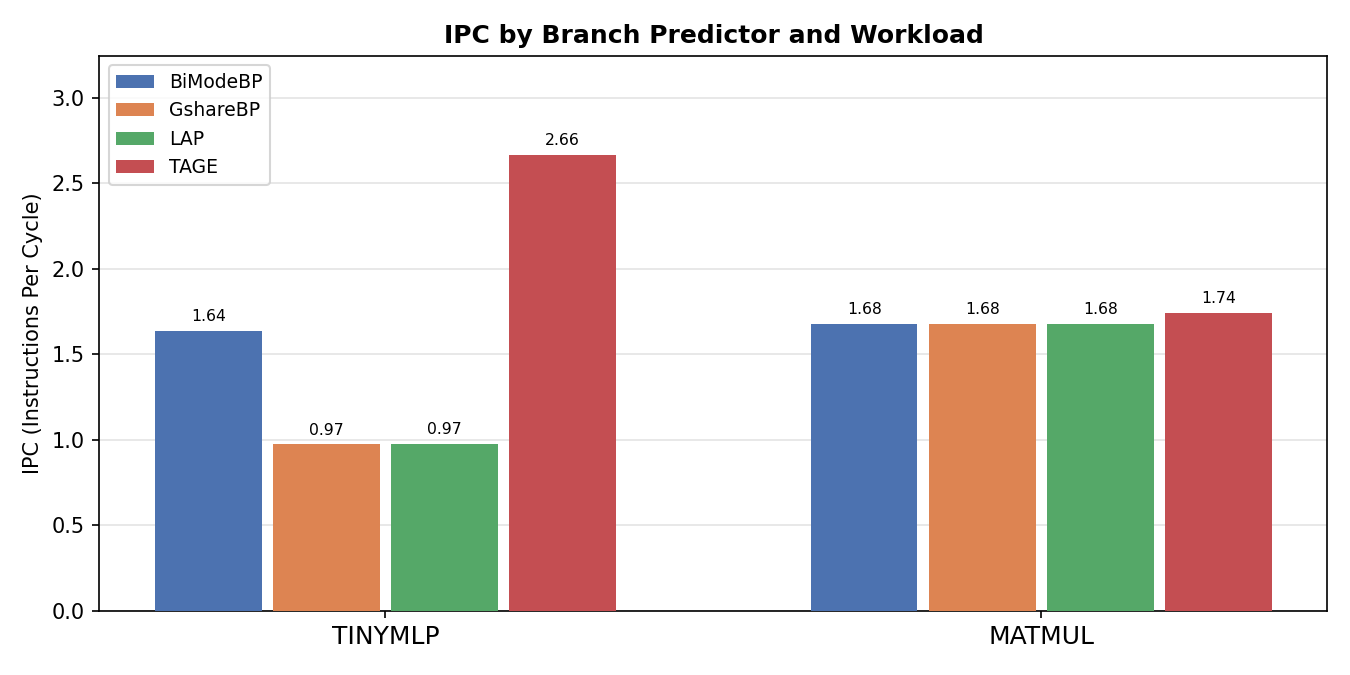
\includegraphics[width=\columnwidth]{results/ipc_comparison.png}
\caption{IPC by branch predictor and workload.}
\label{fig:ipc}
\end{figure}

Figure~\ref{fig:mispred} shows misprediction rates. TAGE is an order of magnitude lower than the baselines on both workloads (0.23\% on \texttt{tinymlp}, 0.05\% on \texttt{matmul}). BiModeBP outperforms GshareBP on \texttt{tinymlp} (5.2\% vs.\ 7.6\%), which is the opposite of the textbook expectation and reflects the heavily biased nature of AI-workload branches. LAP matches GshareBP exactly on \texttt{tinymlp} and is marginally better on \texttt{matmul} (1.57\% vs.\ 1.59\%).

\begin{figure}[t]
\centering
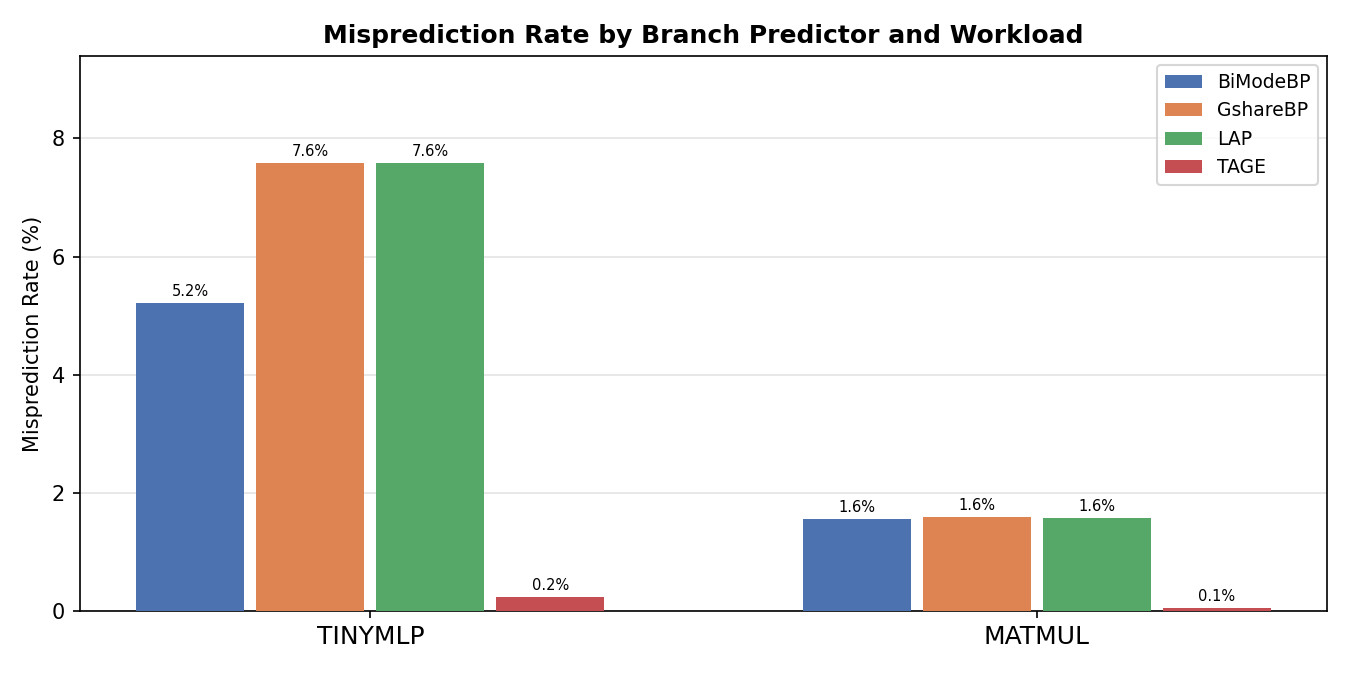
\includegraphics[width=\columnwidth]{results/mispred_comparison.png}
\caption{Misprediction rate (\%) by branch predictor and workload.}
\label{fig:mispred}
\end{figure}

\subsection{Storage Efficiency}

Figure~\ref{fig:storage} plots IPC per kilobyte of conditional predictor storage, a metric that captures the cost--performance trade-off relevant to area- and power-constrained designs. GshareBP dominates this metric on both workloads (1.95 IPC/KB on \texttt{tinymlp}, 3.36 IPC/KB on \texttt{matmul}) because its PHT is only 0.5\,KB. TAGE, despite its absolute IPC advantage, delivers only 0.34 and 0.22 IPC/KB respectively because its tagged tables consume 7.94\,KB. LAP occupies a middle position (0.46 and 0.79 IPC/KB), reflecting its moderate 2.13\,KB footprint.

\begin{figure}[t]
\centering
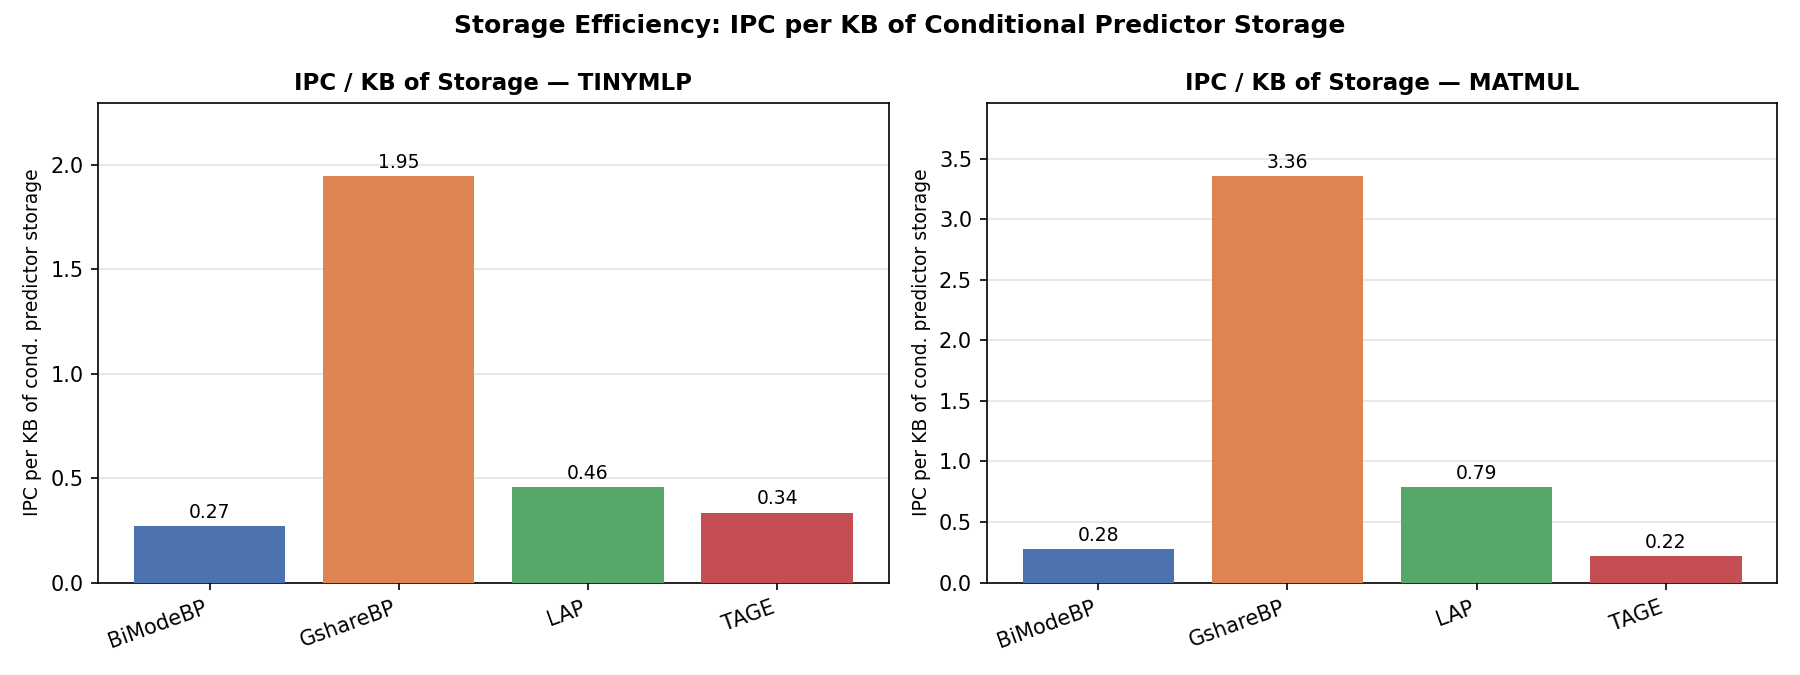
\includegraphics[width=\columnwidth]{results/storage_efficiency.png}
\caption{Storage efficiency: IPC per KB of conditional predictor storage.}
\label{fig:storage}
\end{figure}

\subsection{LABP Loop Predictor Activity}

On \texttt{tinymlp}, the loop component fired only 2{,}677 times across 5.8M lookups, with 2{,}676 correct and 1 wrong. The near-perfect per-use accuracy confirms the loop detector works correctly; the problem is that it rarely activates because \texttt{tinymlp}'s data-dependent branches are not loop-exit branches.

On \texttt{matmul}, the loop component was active for 295{,}612 out of 1.47M lookups (20.1\%), achieving 98.5\% accuracy (291{,}273 correct, 4{,}339 wrong). Figure~\ref{fig:lap_matmul} visualises this activity. The high activation rate and accuracy validate the loop-detection mechanism on a purely loop-dominated kernel.

\begin{figure}[t]
\centering
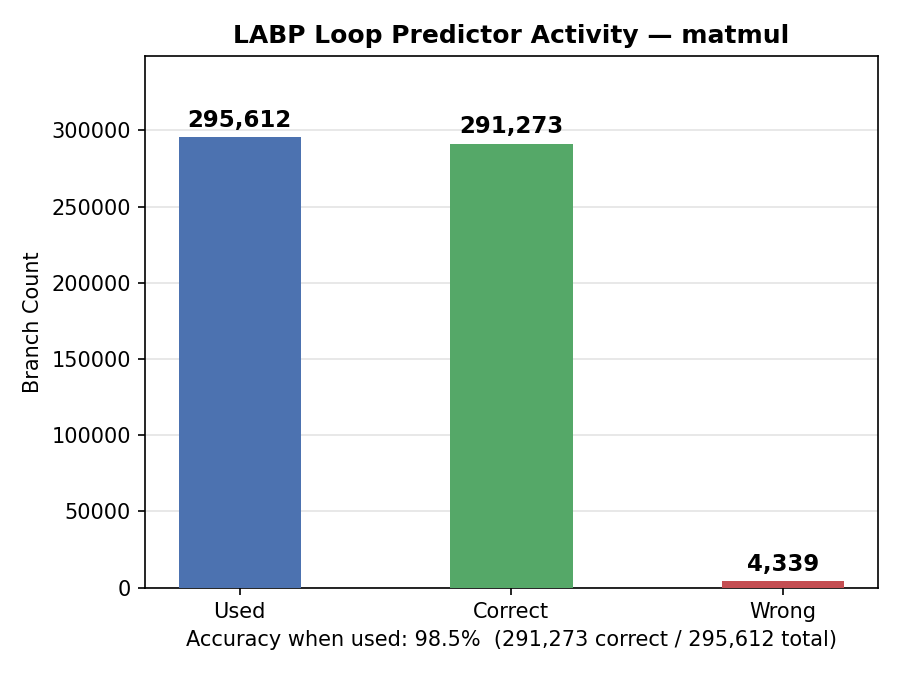
\includegraphics[width=0.85\columnwidth]{results/lap_loop_predictor_matmul.png}
\caption{LABP loop predictor activity on \texttt{matmul}: 295{,}612 loop-override predictions with 98.5\% accuracy.}
\label{fig:lap_matmul}
\end{figure}

\subsection{Analysis}

Three key insights emerge from the results.

First, TAGE remains the strongest design by a wide margin. Its misprediction rate is more than an order of magnitude lower than the simple baselines, and that advantage translates directly into the highest IPC on both workloads. This is expected from the tagged multi-history literature: when branch behavior is heterogeneous, the ability to match multiple correlation lengths and suppress aliasing is decisive~\cite{michaud_2005,seznec_michaud_2006,seznec_2016}. The gap is especially pronounced on \texttt{tinymlp}, where data-dependent branches dominate.

Second, the LABP design \emph{partially} validates the simplification hypothesis, but only on the right workload. On \texttt{matmul}, where the branch stream is almost entirely composed of counted-loop exits, LABP's loop component is active and accurate, and the overall misprediction rate (1.57\%) is slightly lower than both BiModeBP (1.55\%) and GshareBP (1.59\%). On \texttt{tinymlp}, however, LAP matches GshareBP exactly because the loop component almost never activates; the data-dependent sparsity and activation branches simply do not trigger loop detection.

Third, the workload contrast is the most informative finding. The difference between \texttt{matmul} (pure loop nests, high LABP activation) and \texttt{tinymlp} (mixed control flow, negligible LABP activation) demonstrates that branch prediction simplification is \emph{workload-selective}. A simplified loop-aware predictor is viable for kernels whose branch stream is genuinely dominated by regular loop control, but not for workloads where data-dependent conditions constitute a significant fraction of dynamic branches. This implies that deploying a loop-aware predictor in an AI accelerator would require either workload profiling or a conservative fallback strategy to avoid degrading performance on irregular control flow.

\section{Conclusion}

This project investigated whether branch prediction can be simplified for AI workloads by exploiting the regular loop structure that characterises many AI kernels. We implemented a Loop-Aware Branch Predictor (LABP) in gem5 and compared it against BiModeBP, GshareBP, and TAGE on two representative microbenchmarks.

The results show that TAGE remains decisively superior in absolute accuracy and IPC. However, the workload-dependent behaviour of LABP provides a nuanced answer to the research question. On a purely loop-dominated kernel (\texttt{matmul}), the loop component activates frequently and achieves 98.5\% accuracy, demonstrating that loop-aware prediction is a sound mechanism when the branch stream matches the predictor's assumptions. On a mixed-control-flow kernel (\texttt{tinymlp}), the loop component rarely activates, and LABP reduces to its bimodal base, matching GshareBP.

These findings suggest that branch prediction simplification for AI workloads is not a universal opportunity but a workload-selective one. For dense, regular kernels such as matrix multiplication, a lightweight loop-aware predictor can recover most of the available prediction accuracy at substantially lower storage cost than TAGE. For inference workloads with significant data-dependent branching, a more sophisticated predictor remains necessary. Future work should explore adaptive confidence gating, integration with compiler-assisted loop annotations, and evaluation on larger AI workloads including convolutional and attention-based kernels.

\section*{Author Contributions}

\begin{itemize}
    \item \textbf{Simon Darota} (100067950): Led the environment setup and baseline benchmarking phases (Phases~1--2). Installed and configured gem5 for RISC-V, developed and compiled the benchmark workloads (\texttt{tinymlp} and \texttt{matmul}), designed the simulation experiments, ran all baseline predictor evaluations (BiModeBP, GshareBP, TAGE), built the automated analysis pipeline and Jupyter notebook for result extraction and visualisation, and co-authored the report.
    \item \textbf{Winner Abula} (100066896): Led the predictor design and evaluation phases (Phases~3--4). Designed the Loop-Aware Branch Predictor architecture, implemented LABP in the gem5 source tree as a new \texttt{ConditionalPredictor}, ran LABP simulations on both workloads, performed the comparative analysis between LABP and the baselines, documented the predictor design and pseudocode, and co-authored the report.
\end{itemize}

\appendix

\section{Experimental Configuration}
\label{app:config}

All simulations use the following gem5 configuration:

\begin{itemize}
    \item \textbf{ISA:} RISC-V (RV64GC)
    \item \textbf{CPU model:} O3CPU (out-of-order, 8-wide issue)
    \item \textbf{Mode:} Syscall Emulation (SE)
    \item \textbf{L1I/L1D cache:} 32\,KB each, 2-way set-associative
    \item \textbf{L2 cache:} 256\,KB, 8-way set-associative
    \item \textbf{Committed instructions:} 10 million per run
    \item \textbf{Compiler:} \texttt{riscv64-linux-gnu-g++} with \texttt{-O3 -static}
\end{itemize}

\noindent Conditional predictor storage estimates are derived from each predictor's \texttt{config.ini} parameters: table sizes, tag widths, counter bit-widths, and number of entries. For TAGE, all tagged tables are summed; for LABP, the bimodal counters plus loop table entries are included.

\section{Source Code Structure}
\label{app:code}

The project repository is organised as follows:

\begin{itemize}
    \item \texttt{benchmarks/} --- Workload source code and Makefiles for \texttt{tinymlp} and \texttt{matmul}.
    \item \texttt{configs/} --- gem5 Python configuration scripts for SE-mode O3CPU runs.
    \item \texttt{results/} --- Raw \texttt{stats.txt}, \texttt{config.ini}, generated CSV files, and plots.
    \item \texttt{analysis/} --- Jupyter notebook for automated data extraction, table generation, and figure export.
    \item \texttt{gem5/src/cpu/pred/} --- LABP implementation files integrated into the gem5 branch prediction subsystem.
\end{itemize}

\bibliographystyle{IEEEtran}
\begin{thebibliography}{12}

\bibitem{smith_1981}
J. E. Smith, ``A study of branch prediction strategies,'' in \emph{Proc. 8th Annu. Symp. Computer Architecture}, 1981, pp. 135--148.

\bibitem{yeh_patt_1992}
T.-Y. Yeh and Y. N. Patt, ``Alternative implementations of two-level adaptive branch prediction,'' in \emph{Proc. 19th Annu. Int. Symp. Computer Architecture}, 1992, pp. 124--134.

\bibitem{mcfarling_1993}
S. McFarling, ``Combining branch predictors,'' Digital Western Research Laboratory, Tech. Rep. TN-36, 1993.

\bibitem{young_1995}
C. C. Young, N. Gloy, and M. D. Smith, ``A comparative analysis of schemes for correlated branch prediction,'' in \emph{Proc. 22nd Annu. Int. Symp. Computer Architecture}, 1995, pp. 276--286.

\bibitem{michaud_2005}
P. Michaud, ``A PPM-like, tag-based predictor,'' \emph{Journal of Instruction-Level Parallelism}, vol. 7, 2005.

\bibitem{seznec_michaud_2006}
A. Seznec and P. Michaud, ``A case for (partially) TAgged GEometric history length branch prediction,'' \emph{Journal of Instruction-Level Parallelism}, vol. 8, 2006.

\bibitem{seznec_2016}
A. Seznec, ``TAGE-SC-L branch predictors again,'' in \emph{Proc. 5th JILP Workshop on Computer Architecture Competitions}, 2016.

\bibitem{jimenez_lin_2001}
D. A. Jim\'enez and C. Lin, ``Dynamic branch prediction with perceptrons,'' in \emph{Proc. 7th Int. Symp. High-Performance Computer Architecture}, 2001, pp. 197--206.

\bibitem{jimenez_lin_2002}
D. A. Jim\'enez and C. Lin, ``Neural methods for dynamic branch prediction,'' \emph{ACM Trans. Computer Systems}, vol. 20, no. 4, pp. 369--397, 2002.

\bibitem{sutar_guinde_2025}
D. G. Sutar and N. B. Guinde, ``Towards memory-efficient and high-performance branch prediction: the LXOR architecture for control flow optimization in embedded and general-purpose RISC-V processors,'' \emph{Journal of Low Power Electronics and Applications}, vol. 15, no. 4, p. 64, 2025.

\bibitem{vikas_gratz_jimenez_2025}
Vikas, P. Gratz, and D. A. Jim\'enez, ``Workload characterization for branch predictability,'' arXiv:2512.15827, 2025.

\bibitem{ibm_power_2020}
IBM Corporation, ``Performance optimization and tuning techniques for IBM Power Systems processors including IBM POWER8,'' IBM Redpaper REDP-5612, 2020.

\bibitem{gem5_101}
gem5 Project, ``gem5 101,'' [Online]. Available: \url{https://www.gem5.org/documentation/learning_gem5/gem5_101/}

\end{thebibliography}

\end{document}